\chapter{系統架構與方法}
\label{chapter:system}



\section{系統架構}
\label{sec:systemarchi}
本研究專注於透過設計資料庫並用其資料訓練夾取可行性預測系統,並以此作為線索作為雙手臂主動式操作系統的策略因此可分為三大部分:商品語意基準資料庫、夾取可行性預測系統、雙手臂主動式操作系統。基準資料庫目的在設計一個專門給日常商品的資料庫,此資料庫包含物品場景圖片、商品語意如商品整體遮罩、條碼遮罩、品牌文字遮罩,因此可利用這份資料集訓練夾取可行性預測系統,基準資料庫包含參考Amazon Picking Challenge來選取物品、實驗環境設計、並分別搭建現實與虛擬環境以蒐集資料並加以驗證。而夾取可行性預測系統則是改善~\cite{peterthesis}所提出之商品文字姿態估計系統之缺點,並改良成雙手臂夾取可行性預測系統,此系統包含品牌文字、物品語意分割、以及基於語意與三維點雲資訊之夾取可行性預測。而最後的雙手臂主動式操作系統則是設計雙手臂協作方式、手臂功能、假爪選擇與設計、以及最後執行任務之有限狀態機(Finite State Machine)。此系統的設計考量與基準資料庫物品選擇、夾取可行性預測系統環環相扣,因此接下來將先說明環境架設以及主動式操作系統硬體設計,接下來依序說明如何蒐集商品語意基準資料庫、夾取可行性預測系統。最後以主動式操作系統有限狀態機總結整體系統。

\section{硬體架構}
本研究專注於透過設計資料庫並用其資料訓練夾取可行性預測系統,並以此作為線索作為雙手臂主動式操

\begin{figure*}[htb]
   \centering
     \begin{subfigure}[t] {0.43\textwidth}
          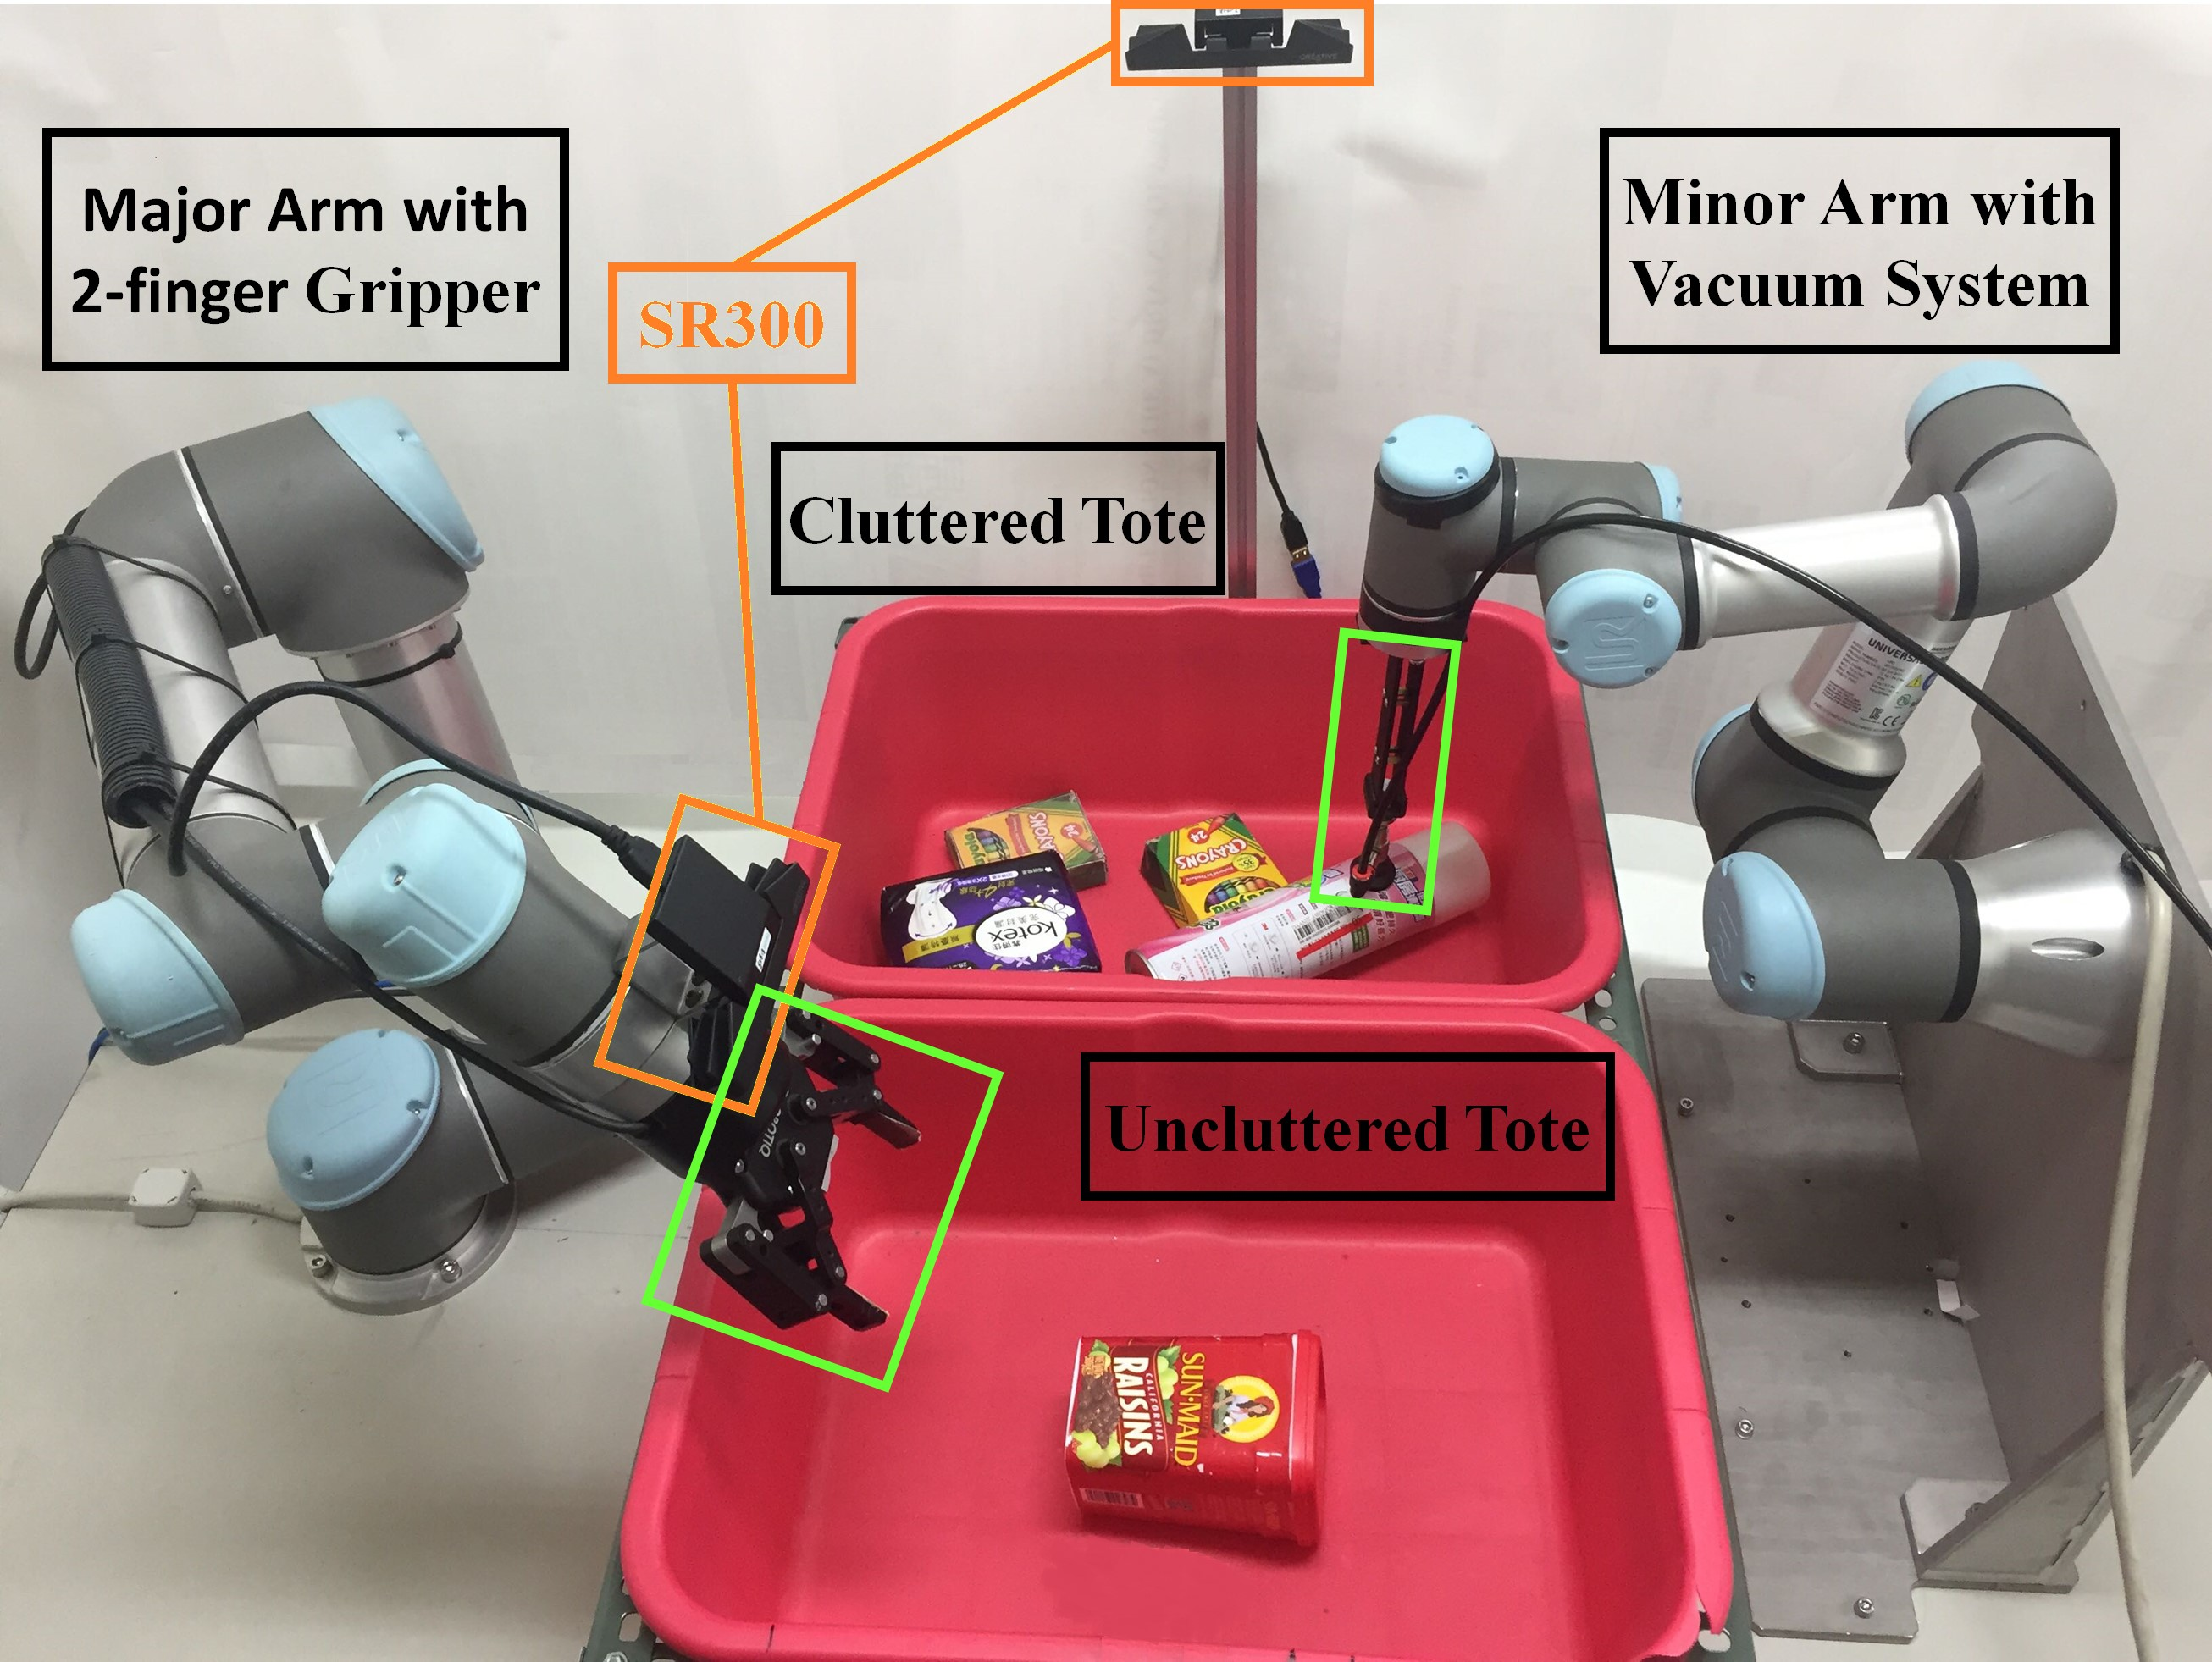
\includegraphics[width=\textwidth]{./figures/robot_system_v2.jpg}
          %\caption{Collaborative robotic arms for pose-aware placing. }
 	\label{fig:robot_system}
      \end{subfigure}
     \begin{subfigure}[t] {0.53\textwidth}
          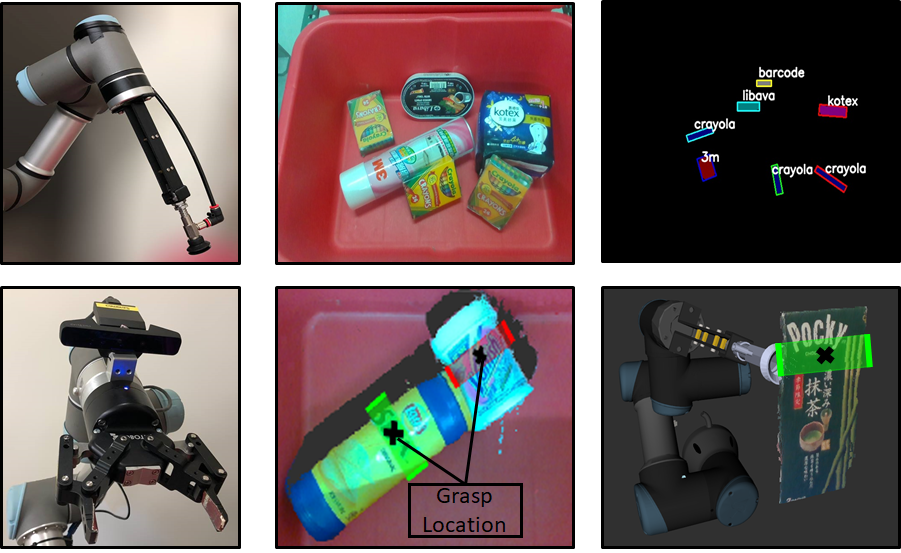
\includegraphics[width=\textwidth]{./figures/affordance_v3.png}
          %\caption{Brandname-based affordance and grasp predictions. }
	\label{fig:brandname-direction}
      \end{subfigure}
   \caption{圖1.左圖:本研究提出雙手臂主動式操作系統去主動改變場景以達到改善機器人感知環境能力,並最佳化物品夾取可行性系統的效果。吸盤假爪從一個雜亂環境移動物品去取得被隱蔽或部分遮蔽的品牌文字資訊。而雙指假爪則藉由基於品牌文字之線索預測夾取點,以此去完成特定姿態的物品擺放任務。右圖:基於品牌文字,本研究可在雜亂環境中預測品牌文字姿態,並以此針對吸盤假爪與雙指假爪進行物品夾取可能性預測。
}
\label{fig:baseline-active}
\end{figure*}

\subsection{多視角主動式視覺}

\subsection{手臂假爪配置}

\section{商品語意資料庫}

\subsection{真實世界訓練集}

\subsection{虛擬世界訓練集}

\subsection{真實世界測試集}

\section{基於品牌文字之夾取可行性預測}

\subsection{品牌文字語意分割}

\subsection{夾取可行性預測}

\section{主動式操作系統}

\subsection{單手臂操作}
本研究專注於透過設計資料庫並用其資料訓練夾取可行性預測系統,並以此作為線索作為雙手臂主動式操

\subsection{夾取可行性預測}
本研究專注於透過設計資料庫並用其資料訓練夾取可行性預測系統,並以此作為線索作為雙手臂主動式操
